\documentclass[conference]{IEEEtran}
\IEEEoverridecommandlockouts
% The preceding line is only needed to identify funding in the first footnote. If that is unneeded, please comment it out.
\usepackage{cite}
\usepackage{amsmath,amssymb,amsfonts}
\usepackage{algorithmic}
\usepackage{graphicx}
\usepackage{textcomp}
\usepackage{xcolor}
\usepackage{amsmath}
\usepackage{booktabs}
\usepackage {multirow}
\usepackage{float}
\renewcommand{\figurename}{Gambar}
\renewcommand{\tablename}{Tabel}
\renewcommand{\IEEEkeywordsname}{Keywords}
\usepackage{caption}
\usepackage{pgf}
\restylefloat{table}
\def\BibTeX{{\rm B\kern-.05em{\sc i\kern-.025em b}\kern-.08em
    T\kern-.1667em\lower.7ex\hbox{E}\kern-.125emX}}
\begin{document}

\title{Tugas 7

MLIDS: A Machine Learning Approach for Intrusion Detection for Real Time Network Dataset\\
{\footnotesize \textsuperscript{}}
\thanks{Identify applicable funding agency here. If none, delete this.}
}
\author{\IEEEauthorblockN{\textsuperscript{} Johnny}
\IEEEauthorblockA{\textit{Institut Teknologi Batam} \\
\textit{Teknologi Informasi}\\
Batam, Indonesia \\
1822004@student.iteba.ac.id}
\and
}

\maketitle

\begin{abstract}
Keamanan jaringan komputer dan mesin virtual sangat penting di era sekarang ini. Berbagai arsitektur telah diusulkan untuk keamanan jaringan atau mencegah akses berbahaya dari pengguna internal atau eksternal. Berbagai sistem yang ada telah dikembangkan untuk mendeteksi aktivitas jahat pada mesin korban; terkadang setiap pengguna eksternal membuat beberapa perilaku jahat dan mendapatkan akses tidak sah dari mesin korban ke sistem perilaku yang dianggap sebagai aktivitas jahat atau Penyusup.Berbagai pembelajaran mesin dan teknik komputasi lunak dirancang untuk mendeteksi aktivitas dalam data audit log jaringan waktu nyata. KKDDCUP99 dan NLSKDD paling banyak menggunakan kumpulan data untuk mendeteksi Penyusup pada kumpulan data benchmark. Dalam makalah ini, kami mengusulkan identifikasi penyusup menggunakan algoritma pembelajaran mesin.Dua teknik berbeda telah diusulkan seperti tanda tangan dengan deteksi dan deteksi berbasis anomali. Dalam analisis eksperimental, menunjukkan SVM, Naive Bayes dan algoritma ANN dengan berbagai set data dan menunjukkan kinerja sistem pada lingkungan jaringan waktu nyata.
\end{abstract}

\begin{IEEEkeywords}
Intrusion Detection System, Network security, Naïve Bayes, SVM, Artificial Neural Network, KDDCUP99.
\end{IEEEkeywords}

\section{PENDAHULUAN}
IDS khusus untuk mendeteksi satu jenis serangan,
misalnya Contoh atau serangan yang tidak diketahui, serangan DoS atau serangan U2R atau serangan R2L.Kemudian secara berurutan menyebarkan sejumlah subsistem tersebut, satu per satu. Ini memiliki dua tujuan: pertama, hanya sejumlah fitur yang mendeteksi jenis serangan tertentu yang dapat dilatih di setiap sub-fase. Kedua, perangkat sub-ukuran tetap kecil dan karena itu berfungsi. Mirip dengan skema kami, kelemahan umum adalah meningkatkan komunikasi overhead antar modul.

Metode mendefinisikan sistem untuk membuat aturan SVM dalam pekerjaan penelitian ini, berdasarkan prosedur pemilihan perannya, yang bekerja pada HIDS dan NIDS. Algoritma genetika adalah algoritma optimasi yang digunakan untuk mencari solusi terbaik.Untuk semua jenis sub-serangan kelas master, pendekatan ensemble dengan algoritma klasifikasi yang berbeda dapat memberikan deteksi NIDS terbaik.

\section{PEMBHASAN}

Bhosale, Karuna S. et al. [1] \cite {bhosale2018modified} deep neural network (DNN), Membuat IDS yang terukur dan efisien untuk mengenali dan mengenali serangan cyber yang tidak disengaja dan tidak terduga dipelajari sebagai bentuk sistem pembelajaran mendalam. Perubahan konstan dalam operasi jaringan dan penciptaan serangan yang cepat melibatkan peninjauan kejadian yang sering terjadi selama bertahun-tahun melalui teknik dinamis dan statis.

Chamou et al. [2] \cite {chamou2019intrusion}, Karena penjelasan itulah komunitas sains telah terbiasa dengan kompleksitas dan peningkatan efisiensi sistem deteksi intrusi sehingga sejumlah besar perusahaan di seluruh dunia menjadi sasaran dan terancam oleh munculnya ancaman baru dan yang muncul terus-menerus. Ini adalah alat inovatif untuk mengevaluasi aktivitas mencurigakan di DDoS dan ancaman cyber malware menggunakan model pembelajaran mendalam.

According to [3] \cite {anbar2016comparative}, sebuah sistem telah dikembangkan untuk secara akurat mendeteksi potensi serangan dengan menggunakan berbagai bebas keputusan, hutan acak, dan KNN. Teknik baru disarankan untuk memperbaiki kekurangan dari pendekatan sebelumnya yang tidak dapat mendeteksi serangan IPv6. Dalam mendeteksi serangan berbasis IPV4, kerangka kerja yang ditetapkan menghasilkan hasil yang mengesankan dan efisien, dengan mempertimbangkan kemungkinan jangkauan—efisiensi dari berbagai algoritme yang telah diukur. 

According to [4] \cite {chen2017novel}, mengidentifikasi fenomena baru yang disebut NEC, clustering, dan KDD dapat digunakan secara efektif. Anomali tanpa pengawasan digunakan untuk menghasilkan tingkat deteksi yang tinggi dan tingkat pasif palsu yang lebih sedikit. Ini adalah cara yang efektif untuk memecahkan masalah dan menemukan anomali yang tidak melibatkan pengumpulan data berlabel.

Machine Learning Survey[5] \cite {buczak2015survey}. Untuk mengakses header paket dan header paket aliran bersih digunakan ke jaringan dan data tingkat kernel untuk proses deteksi intrusi, masalah potensial adalah bahwa penambangan data dan kecerdasan buatan tidak dapat dicapai tanpa database aktual, oleh karena itu, sangat memakan waktu. Kehadiran berbagai statistik dan algoritma pembelajaran mesin dibahas. Makalah penelitian berisi serangkaian kriteria komparatif untuk anomali metodologi untuk penambangan data pembelajaran mesin — deteksi intrusi dependen membantu menemukan, mengevaluasi, dan mengenali penggunaan, replikasi, perubahan, dan penghancuran sistem informasi yang tidak sah.

Based on the [6] \cite {koli2017advanced}, deteksi dan pemantauan penyusup menggunakan pembelajaran mesin, peringkat, dan Voronoi, keamanan telah ditingkatkan.

According to ADS-B IDS[7] \cite {kacem2016ads}, teknik IDS pengawasan-siaran berbasis otomatis diusulkan menggunakan teknik ADS-B. Untuk meningkatkan kinerja kontrol lalu lintas udara, kumpulan data HMAC digunakan. Pendekatan beroperasi dengan overhead minimum. Cakupan mendatang menetapkan bahwa jaraknya dari posisi satu kali yang sesuai berada dalam zona aman untuk lokasi ADS-B agar valid. GPS menggunakan lingkungan fisik-cyber yang divalidasi oleh deteksi serangan untuk menentukan spesifikasi radar di pesawat yang memberi sinyal presisi lokasi yang unggul, karena ADS-B telah muncul sebagai alternatif radio saat ini. Sebuah protokol disarankan untuk menukar kunci yang digunakan untuk algoritma HMAC dengan aman.

According to [8] \cite {pan2015developing}, untuk perangkat listrik yang mendukung data log, laporan tersebut menyatakan bahwa kombinasi IDS menggunakan data mining dibuat menggunakan proses penambangan yang aman. Metode tersebut merupakan pendekatan terpadu untuk merancang prototipe IDS. Ketepatan deteksi, yang mencapai 73 persen, telah menjadi salah satu keunggulan utama. Tetapi pendekatan ini tidak cukup untuk mengumpulkan isu-isu utama seperti log data, meskipun rumit. Kerangka kerja ini memanfaatkan fungsionalitas IDS berbasis karakteristik dan spesifikasi. Metodologi analisis data yang menggabungkan log audit untuk mempelajari rute umum dari perangkat mesin yang berbeda.

According to Al, Dr. Yogesh Kumar Sharma et.[9] \cite {borole20206g} mendefinisikan sistem Akses Jaringan 6G dan Mekanisme Aturan Congestion Edge-Assisted menggunakan Jaringan yang Ditentukan Perangkat Lunak Untuk menghindari buffering arus lalu lintas, kerangka kerja harus menggunakan data frekuensi besar.

\section{METODOLOGI}
Metodologi penelitian yang diusulkan melakukan deteksi dan pencegahan intrusi menggunakan teknik pembelajaran mesin. Pelatihan, termasuk pilihan paket untuk anomali dan pemantauan jarak jauh, akan dilakukan oleh lingkungan paket yang dicirikan blok Kemudian akan mengirimkan kumpulan fungsi untuk aktivitas paket tertentu. Jika semuanya baik-baik saja, kirimkan bersama-sama. Untuk mendeteksi serangan individu, sampel perilaku buruk akan diuji untuk pemilihan fitur untuk berbagai
kualitas. Ada dua fase dalam sistem yang diusulkan; kami telah mengambil dataset jaringan untuk tujuan pelatihan dan pengujian sistem—komponen kerangka kerja.

Kumpulan data NSL KDD CUP 1999 digunakan untuk eksperimen (kumpulan data KDD, 1999). Dataset KDD CUP 1999 adalah versi perangkat lunak penilaian deteksi intrusi DARPA 1998 asli milik MIT Lincoln Laboratory, yang siap dan terkontrol.Semua jenis kontinu, diskrit,dan variabel simbolik memiliki opsi ini, dengan rentang yang sangat bervariasi jatuh ke dalam empat kategori:

(1) kelas utama terdiri dari opsi intrinsik asosiasi, termasuk opsi kritis untuk menghubungkan protokol kontrol transmisi individu. Berbagai pilihan termasuk panjang afiliasi, jenis protokol (TCP, UDP, dll.), dan unit area akses jaringan (HTTP, telnet, dll.).

(2) Pilihan konten dalam asosiasi yang diberitahukan oleh Unit Area Data Domain, seperti jumlah upaya login yang gagal, tidak akan menentukan muatan paket protokol kontrol transmisi pertama. 

(3) Opsi host konstan menganalisis koneksi yang ditentukan yang memiliki host tujuan berkelanjutan dalam 2 detik terakhir karena hubungan saat ini dan mengukur statistik yang terkait dengan perilaku protokol, operasi, dll.

(4) Opsi layanan serupa memeriksa koneksi yang memiliki layanan yang sama dengan tautan saat ini dalam dua detik terakhir.

\begin{figure}
\centering
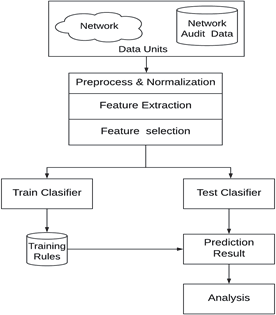
\includegraphics[width=.3\textwidth]{Gambar/pct1.png}
\caption{System architecture}
\end{figure}

Pada titik pra-pemrosesan, blok kedua dari Gambar 1 menunjukkan bahwa kita menggunakan packet sniffer yang dirancang dengan perpustakaan winpcap untuk mengekstrak informasi paket jaringan dari setiap paket, termasuk header IP, header TCP, header UDP, dan header ICMP. Setelah itu, dengan mempertimbangkan hubungan antara setiap kombinasi alamat sains (ilmu sumber dan IP tujuan), paket data dipartisi dan dibentuk menjadi catatan dengan menggabungkan setiap informasi.

\section{HASIL DAN DISKUSI}

Setelah implementasi sistem berhasil, kami menghitung matriks kebingungan untuk sistem. Tabel 1 dan Tabel 2 menunjukkan klasifikasi dengan algoritma SVM. Angka
2 menunjukkan kinerja klasifikasi pengumpulan data oleh KDDCUP menggunakan pendekatan berbasis kepadatan dari program algoritma pembelajaran mesin Gambar 3 digunakan untuk mengklasifikasikan dan memprediksi presisi sistem menggunakan
metode yang berbeda seperti algoritma RNN.

\subsection{TABEL 1 (CONFUSION MATRIX CALCULATION USING SVM FOR CLASSIFICATION)}

\begin{table}[H]
\begin{tabular}{|c|c|c|c|}
\hline
no & class & normal & Attack\\
\hline
1   & normal & 1760 & 19\\
\hline
2   & attack & 9 & 1640\\
\hline
3   &  & 1769 & 1659 \\
\hline
\end{tabular}
\end{table}

\subsection{TABLE II (CONFUSION MATRIX CALCULATION USING NB FOR CLASSIFICATION)}

\begin{table}[H]
\begin{tabular}{|c|c|c|c|}
\hline
no & class & normal & Attack\\
\hline
1   & normal & 1830 & 227\\
\hline
2   & attack & 169 & 1202\\
\hline
3   &  & 1999 & 1429 \\
\hline
\end{tabular}
\end{table}

\subsection{TABLE III (PERFORMANCE EVALUATION WITH NB AND SVM)}

\begin{table}[H]
\begin{tabular}{|c|c|c|c|}
\hline
no &  & NB & SVM\\
\hline
1   & Accuracy & 0.9892 & 0.9525\\
\hline
2   & Precision & 0.9867 & 0.9797\\
\hline
3   & Recall & 0.9933 & 0.9463 \\
\hline
4   & F-Score& 0.9899 & 0.9529 \\
\hline
\end{tabular}
\end{table}

Menurut kedua analisis eksperimen, SVM menunjukkan akurasi klasifikasi yang lebih baik daripada algoritme NB, yang ditunjukkan pada gambar 3. Berdasarkan analisis eksperimen di atas, kita dapat menyimpulkan bahwa sistem menghasilkan akurasi yang lebih baik untuk komputasi kepercayaan di lingkungan in-service IoT. Seluruh penelitian mengikuti beberapa parameter lingkungan simulasi serta kombinasi dari algoritma pembelajaran mesin.

\begin{figure}
\centering
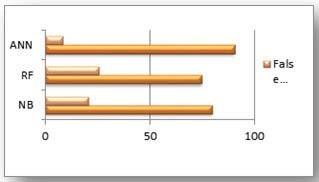
\includegraphics[width=.3\textwidth]{Gambar/pct2.jpg}
\caption{Detection accuracy for KDD : CUP99 dataset using machine learning}
\end{figure}

Gambar 2 di atas Menunjukkan akurasi klasifikasi hasil kddCup 99, dengan lima kelas yang berbeda. Rata-rata keluaran perangkat lunak sekitar algoritma untuk pembelajaran mesin 88,50 percent untuk semua kelas.

\begin{figure}
\centering
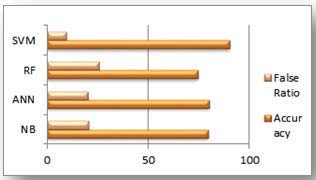
\includegraphics[width=.3\textwidth]{Gambar/pct3.jpg}
\caption{Detection accuracy various network dataset using propsoed (SVM) vs exisitng}
\end{figure}

Gambar 3 di atas menunjukkan efisiensi rata-rata identifikasi di berbagai database, dari (n) kelas yang berbeda. Performa rata-rata sistem dengan algoritme pembelajaran mesin adalah sekitar 95 percent untuk semua (n) kelas

\section{KESIMPULAN}

Studi ini mengusulkan pendekatan SVM-IDS berdasarkan pembelajaran mendalam untuk menyarankan sistem ID yang efisien. Untuk menguji akurasi deteksi anomali, kami menggunakan dataset intrusi berbasis sintetis - NSL-KDD. Kami berencana untuk mengimplementasikan IDS ke lingkungan cloud di masa mendatang menggunakan teknik pembelajaran mendalam. Kami juga menganalisis dan membandingkan berbagai metode deep learning, yaitu. Untuk mendeteksi intrusi dalam jaringan, NB ANN, RF, dan SVM pada dataset NSL-KDD; Program ini pada dasarnya bertindak sebagai algoritma kecerdasan buatan dan pengkondisian untuk menentukan contoh yang tidak diketahui selama pemeriksaan data. Struktur aturan yang efisien menghasilkan klasifikasi yang lebih baik dan deteksi kelas tinggi. Berbagai eksperimen menggunakan analisis eksperimental untuk menilai efisiensi algoritme menggunakan beberapa tes dan menyimpulkan bahwa kami mencapai hasil yang memuaskan.


\bibliographystyle{IEEEtran}
\bibliography{pustaka.bib}
\vspace{12pt}
\end{document}
